% !TEX root = ../../mat701_notes.tex
\newpage
\section{Lebesgue Outer Measure}

We want to assign a notion of `size' to sets. We denote this `size' by $\nu$. Let $\R^n= \{(x_1,\ldots,x_n) \colon x_i \in \R\}$ denote ordinary Euclidean space. By an `interval' in $\R^n$, we mean a set $\{ (a_1,b_1) \times (a_2,b_2) \times \cdots \times (a_n,b_n) \colon a_i,b_i \in \R^n, a_i<b_i\}$. By a closed interval in $\R^n$, we mean a set $\{ [a_1,b_1] \times [a_2,b_2] \times \cdots \times [a_n,b_n] \colon a_i,b_i \in \R^n, a_i<b_i\}$. We will often say `box', which will always mean an open or closed interval in $\R^n$. 
	\[
	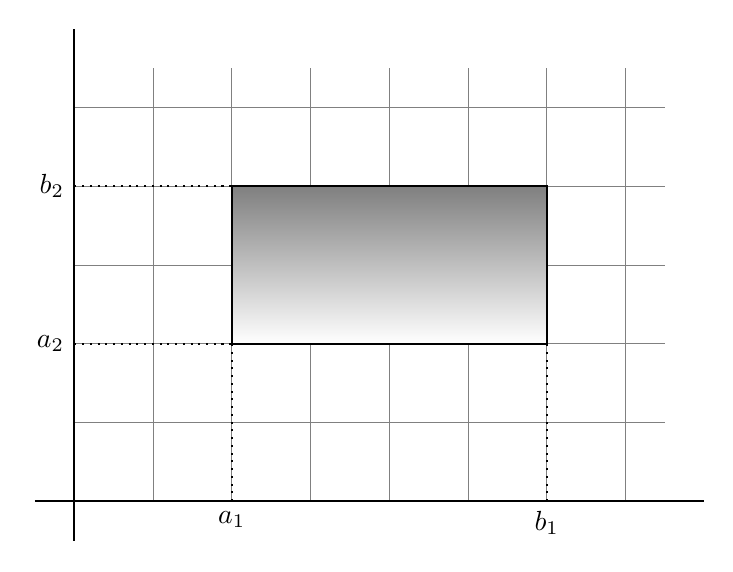
\begin{tikzpicture}[thick]
	\draw[gray,very thin] (0,0) grid (7.5,5.5);
	\draw (0,-0.5) -- (0,6);
	\draw (-0.5,0) -- (8,0);
	\shadedraw (2,2) -- (6,2) -- (6,4) -- (2,4) -- (2,2); % \draw[fill=gray!15]
	\draw[dotted] (2,0) -- (2,2);
	\draw[dotted] (6,0) -- (6,2);
	\draw[dotted] (0,2) -- (2,2);
	\draw[dotted] (0,4) -- (2,4);
	\node[below] at (2,0) {$a_1$};
	\node[below] at (6,0) {$b_1$};
	\node[left] at (0,2) {$a_2$};
	\node[left] at (0,4) {$b_2$};
	\end{tikzpicture}
	\]
In defining a `size' for sets, it makes sense to begin with a simple shape like a box. In the case of the plane, we know the a good notion of size is the area, and the area of a box $[a_1,b_1] \times [a_2,b_2]$ is $(b_1-a_1) \cdot (b_2-a_2)$. We can immediately generalize this to $\R^n$ as follows: if $I \subset \R^n$ is an interval, then we define
	\[
	\nu(I):= \prod_{j=1}^n (b_j - a_j)= (b_1-a_1)(b_2-a_2) \cdots (b_n-a_n)
	\]


\noindent But the question remains, how do we generalize this to an arbitrary region $E$? Given the above definition, it is natural to try to generalize to arbitrary sets $E$ by approximating $E$ by boxes, i.e. an open covering $\{I_k\}$ by intervals.
	\[
	\begin{scaletikzpicturetowidth}{0.3\textwidth}
	\begin{tikzpicture}[thick,scale=\tikzscale]
	\blobfive{0}{0}
	\pbox{-4.5}{-3}{3}{5}
	\pbox{-6.5}{-3.5}{2.5}{3.5}
	\pbox{-2}{2.5}{2}{5}
	\pbox{-4}{-0.5}{3.5}{3.5}
	\pbox{2}{-1.5}{4.5}{2.5}
	\pbox{-1}{-2}{5.5}{3.5}
	\pbox{-2.5}{-3.5}{2}{3.5}
	\end{tikzpicture}
	\end{scaletikzpicturetowidth}
	\]


It then becomes clear that whatever the measure of $E$ is, it should satisfy
	\[
	\nu(E) \leq \sum_k \nu(I_k),
	\]
since the intervals cover $E$. After all, it would be strange indeed to allow $E$ to have greater measure than its covering. Furthermore measure is going to be defined in terms of coverings, then the measure need be invariant of the choice of covering. These ideas are our guiding principles. So we take the following definition 


\begin{dfn}[Outer Measure]
For a set $E \subset \R^n$, the outer measure (or exterior measure) of $E$, denoted $\ext{E}$, is the function $\nu: \R^n \to [0,\infty)$ given by
	\[
	\ext{E}:= \inf_{E \subset \cup_k I_k} \sum \nu(I_k),
	\]
where the infimum is taken over all \emph{countable} coverings $\{I_k\}$ of $E$. 
\end{dfn}


The coining of `outer measure' is immediately obvious---we are measuring the size of a set via external objects, namely the open cover. However, less obvious is the need to restrict to countable coverings. The need to eliminate uncountable coverings is apparent as then trouble arises defining the summation. But why not only allow finite coverings? For this consider the case $E= \Q \cap [0,1]$. In any finite covering of $[0,1]$ by intervals, the intervals cannot all be pairwise disjoint. The reader will confirm, with a bit of thought, that if the intervals were all pairwise disjoint then there would be a rational number missed by the `covering.' But this contradicts the fact that the collection was an open cover. The the only possible open covering by intervals is the entire interval itself so that $\inf \sum \nu(I_k)=1$. This violates the notation that there isn't any `length' or `area' here since we have a sparse collection of points. 


Furthermore, the same logic applies to the set $E'=\Q^C \cap [0,1]$. So if the outer measure of $E$ were 1, then this would be true too of $E'$. But clearly the outer measure of $[0,1]$ is 1. Now $[0,1]=E \cup E'$, and $E \cap E'=\emptyset$. As $1+1 \neq 1$, this breaks countable subadditivity of the measure we are trying to define. By defining the outer measure in terms of countable covers, we obtain the expected answer $\ext{E}=0$. 


\begin{ex}
Let $E=\Q \cap [0,1]$ and $\ep>0$ be given. Since $\Q$ is countable, so too is $E$ countable. Enumerate the rationals in $E$ as $\{q_1,q_2,\ldots,q_n,\ldots\}$. Now the set $\{O_n\}_{n \in \N}$, where $O_n:= (q_n- \frac{1}{2^{n+k+1}}, q_n+\frac{1}{2^{n+k+1}})$ and $k \in \N$ is fixed, is a (countable) open covering of $E$ by intervals. Furthermore, the $O_n$ are pairwise disjoint. Choose $k$ sufficiently large so that $2^{-k}<\ep$. The measure of this covering is then
	\[
	\sum_{n=1}^\infty \nu(O_n)= \sum_{n=1}^\infty \left[ \left(q_n+\frac{1}{2^{n+k+1}}\right) - \left(q_n- \frac{1}{2^{n+k+1}}\right) \right]= \sum_{n=1}^\infty 2 \cdot \dfrac{1}{2^{n+k+1}}= \dfrac{1}{2^k} \sum_{n=1}^\infty \dfrac{1}{2^n}= \dfrac{1}{2^k}<\ep.
	\] \xqed
\end{ex}


As a final remark, observe that the exterior measure is a function to the nonnegative extended real line; that is, the exterior measure allows infinite values. Sets with an infinite exterior measure are considered measurable. For example, our intuition is that $\R$ should have infinite length and the reader routinely verifies that $\ext{\R}=\infty$. The outer measure $\ext{\cdot}$ defined above does meet all our guiding principles as the following proposition verifies. 

\begin{prop} \label{prop:outermprop} \hfill
	\begin{enumerate}[(i)]
	\item $\nu(\emptyset)=0$.
	\item Monotonicity: if $E_1 \subset E_2$, then $|E_1|_e \leq |E_2|_e$.
	\item Countable Subadditivity: $\displaystyle \ext{\bigcup_{k=1}^\infty E_k} \leq \sum_{k=1}^\infty |E_k|_e$
	\end{enumerate}
\end{prop}

\pf \\
\noindent$(i)$ This holds essentially by fiat. \\

\noindent$(ii)$ This follows immediately from the fact that we are taking an infimum and any open cover of $E_2$ is an open cover of $E_1$. \\

\noindent$(iii)$ Let $E:=\ext{\bigcup_{k=1}^\infty E_k}$. If any of the $E_k$ have infinite exterior measure, the result is immediate. Assume then that $\ext{E_k}<\infty$ for all $k$. Choose $\ep>0$ and cover each $E_k$ by intervals $\{I_n\}$ such that $\sum_n \nu(I_n) \leq \ext{E_k} + \ep/2^k$. Then $E \subset \bigcup_{k,n} I_{k,n}$ and $\ext{E} \leq \sum_{k,n} \nu(I_{k,n})= \sum_k \sum_n \nu(I_{k,n})$. But then 
	\[
	\ext{E} \leq \sum_k \left( \ext{E_k} + \ep/2^k \right)= \ep + \sum_{k=1}^\infty |E_k|_e.
	\]
The result then follows by letting $\ep$ tend to 0. \qed \\


\noindent If one wants to generalize the notion of outer measures to spaces beyond $\R^n$, one can take the properties of Proposition~\ref{prop:outermprop} as the axioms for this abstract measure. 


Note in general we do not have $\ext{\bigcup E_k}= \sum \ext{E}$ even if the $E_k$ are disjoint or even in the case of finite unions! Equality holds when the sets are, in a sense, `unentangled.' By this, we mean that open coverings of one set tend to be disjoint from open coverings of the other set. If this is the case, the sets have to be covered separately, see the example on the left below. However if the sets are `entangled', then their open covers result in a great deal of `multiple-covering' for the union. This excess covering allows one to more `efficiently' cover the union---hence the smaller measure, see the example on the right below. 
	\[
	\begin{scaletikzpicturetowidth}{0.5\textwidth}
	\begin{tikzpicture}[thick,scale=\tikzscale]
	\blobfour{-3}{3}
	\blobseven{7}{-1}
	\pbox{-6}{0.5}{7}{3.5}
	\pbox{-8.5}{-1.5}{4.5}{3.5}
	\pbox{-3}{4.5}{2}{3.7}
	\pbox{-4}{1.5}{3.5}{4.2}
	\pbox{7}{0}{1.6}{4}
	\pbox{2}{0}{2}{3}
	\pbox{4}{-2}{3}{2}
	\pbox{4.5}{-4.5}{4}{4}
	\pbox{4.8}{-1}{3.3}{2.6}
	\pbox{6.5}{-2}{2.3}{5.6}
	\pbox{0.5}{-5.5}{6.2}{5}
	\end{tikzpicture}
	\end{scaletikzpicturetowidth}
	\]


There are many connections between Topology and Measure Theory, especially in the case of $\R^n$. Topology on $\R^n$ is primarily interested in the structure of open and compact sets. This will prove useful for us since our measure is defined in terms of open sets. As an example, take the following theorem. 


\begin{thm} \label{thm:closeopenset}
For all $E \subset \R^n$ and $\ep>0$, there exists an open set $G$ such that $E \subset G$ and $|G|_e \leq |E|_e + \ep$.
\end{thm}

\pf Every interval $I$ is contained in the interior of a slightly larger interval $I'$, i.e. $I \subseteq \inter(I')$, where $\nu(I')  - \nu(I)<\ep$. Take $I_k$ such that $\sum_k \nu(I_k) \leq |E|_e + \ep/2$, and find $I_k'$ such that $I_k \subset \inter (I_k')$ and $\nu(I_k') < \nu(I_k) + \ep/2^{k+1}$. Let $G= \bigcup_k \inter(I_k')$. By construction, $G$ is an open set containing $E$. To complete proof, observe
	\[
	\ext{G} \leq \sum_{k=1}^\infty \nu(I_k') \leq \sum_{k=1}^\infty \nu(I_k) + \ep \sum_{k=1}^\infty \dfrac{1}{2^{k+1}} \leq \ext{E} + \ep.
	\] \qed \\


\begin{cor} \label{cor:gdeltaclose}
For every set $E$, there exists a $G_\delta$ set $G$ such that $E \subset G$ and $|E|_e=|G|_e$.
\end{cor}


\begin{cor} \label{cor:countmeasurezero}
Any subset of a set with outer measure zero has outer measure zero, and the countable union of sets with outer measure zero has outer measure zero. In particular, any countable set has outer measure zero. 
\end{cor}


Theorem~\ref{thm:closeopenset} says we can always approximate any set by an open set with approximately the same size, i.e. approximately the same exterior measure. However, this does not mean that $|G \sm E|_e \leq \ep$. We do know that $G = E \cup (G\sm E)$. By subaddivitivity, we have $|G|_e \leq |E|_e + |G \sm E|_e$. But we do not know the measure of the second set. The set $G$ from Theorem~\ref{thm:closeopenset} is a special case of more general type of set.


\begin{dfn}[$G_\delta$-Set]
A $G_\delta$ set is a countable intersection of open sets. 
\end{dfn}

\noindent Notationally, $G$ is because the set is open, and $\delta$ stems from the fact we are using an intersection.


However, it is still important to note that $|G \sm E|_e$ could be very large. Now while Corollary~\ref{cor:countmeasurezero} states that countable sets have outer measure zero, it need not be the case that uncountable sets need have positive measure. 


\begin{ex}[Cantor Set] \label{ex:cantor}
Begin with the closed unit interval $C_0:=[0,1]$. From this interval, remove the middle third, i.e. $(\frac{1}{3},\frac{1}{3})$, and label $C_1:=[0,\frac{1}{3}] \cup [\frac{2}{3},1]$. Inductively construct $C_n$ by removing the middle third of each closed subinterval of $C_{n-1}$. We define the Cantor Set by defining $C:= \lim_{n \to \infty} C_n$. The first few stages of the construction of $C$ are shown below. The fact that the Cantor set is uncountable follows from the fact that it is a nonempty compact set without isolated points.
	\[
        \begin{tikzpicture}[decoration=Cantor set,line width=1mm]
        \draw (0,0) -- (3,0);
        \draw decorate{ (0,-.5) -- (3,-.5) };
        \draw decorate{ decorate{ (0,-1) -- (3,-1) }};
        \draw decorate{ decorate{ decorate{ (0,-1.5) -- (3,-1.5) }}};
        \draw decorate{ decorate{ decorate{ decorate{ (0,-2) -- (3,-2) }}}};
        \end{tikzpicture}
        \]
What is $\ext{C}$? Note that $C_n$ is the union of $2^n$ intervals, each having length $1/3^n$, and that $C \subset C_n$ for all $n \in \N$. But then the Cantor set is contained in a union of $2^n$ intervals with length $1/3^n$, which has total length $2^n \cdot 1/3^n= (2/3)^n$. The fact that $\ext{C}=0$ is then clear as $\lim_{n \to \infty} (2/3)^n=0$.  \xqed
\end{ex}


\begin{lem} \label{lem:fincovcomset}
If $K \subset \R^n$ is compact, then $\ext{K}= \inf \left\{ \sum_k \nu(I_k) \colon \{I_k\} \text{ finite cover of }K \right\}$. 
\end{lem}

\pf Let $\ep>0$. By Theorem~\ref{thm:closeopenset}, every interval is contained some set $\interior(I')$, where $\nu(I')< \nu(I) + \ep$. Given a countable cover $I_k$ of $K$, choose $I_k'$ such that $I_k \subset \interior(I_k')$ and $\nu(I_k') < \nu(I_k) + \ep/2^k$. Then $\{\interior(I_k')\}_k$ is an open cover for $K$, so there exists a finite subcovering $\{I_{k,n}\}_{n=1,\ldots,N}$. Therefore, we have $K \subset \bigcup_j I_{k,j}'$. By countable subadditivity,
	\[
	\sum_{n=1}^N \nu(I_{k,n}') < \ep + \sum_{n=1}^N \nu(I_k),
	\]
as desired. \qed \\


\begin{prop}
$\ext{[a,b]}= b-a$. 
\end{prop}

\pf Clearly, $\ext{[a,b]} \leq b-a$, so it remains to show that $b-a \leq \ext{[a,b]}$. Suppose that $[a,b]$ is a finite union of intervals of the form $[c_j,d_j]$. There exists $j_1$ such that $c_{j_1} \leq a$. If $d_{j_1} \geq b$, then $\ext{[a,b]} \geq d_{j_1} - c_{j_1} \geq b-a$, and we are done. Otherwise, it must be that $d_{j_1} < b$. There then exists $j_2$ such that $c_{j_2} \leq d_{j_1}$. Continue this process inductively until one finally obtains $d_{j_r} \geq b$. But then taking the sum of these differences, one obtains a telescoping series
	\[
	\underbrace{(d_{j_{r}} - c_{j_{r}})}_{\geq 0} + \underbrace{(d_{j_{r-1}} - c_{j_{r-1}})}_{\geq 0} + \cdots + \underbrace{(d_{j_{1}} - c_{j_{1}})}_{\geq 0} \geq b-a.
	\]
\qed \\


More generally, $\ext{I} = \nu(I)$ for all intervals in $\R^n$ and $\ext{\bigcup_{k=1}^N I_k}= \sum_{k=1}^N \nu(I_k)$, provided the $I_k$ are non-overlapping intervals, i.e. $\interior(I_k) \cap \interior(I_j)= \emptyset$. 


%images Boxes kissing, ok. boxes overlap, not so much


\noindent The proof of this is rather ugly---an exercise in making `obvious' geometric facts obvious, and an exercise in bookkeeping---and we shall not concern ourselves with it. We now can define our notion of measurability with our notions of exterior measure firmly in place. 


\begin{dfn}[Measurable]
A set $E \subset \R^n$ is measurable if for all $\ep>0$, there exists an open set $G$ such that $G \supset E$ and $\ext{G \sm E} < \ep$.
\end{dfn}

Essentially, a set is measurable if it can be well approximated by open sets. We choose the above notion of `closeness' in order to obtain additivity of measures. Notice we also have mentioned the underlying topology via the use of `open.' We are able to avoid invoking the underlying topology using greater abstraction, which shall come later. Note that we always have an open set such that $\ext{G} < \ext{E}+\ep$ (c.f. Theorem~\ref{thm:closeopenset}), but this alone is weaker than the above definition; that is, if $E$ is measurable then it satisfies the properties in Theorem~\ref{thm:closeopenset}. As a matter of notation, if $E$ is measurable, we define $|E|:= \ext{E}$. The following propositions follow immediately from our definition.

\begin{prop} \label{prop:openmeasurable}
Every open set is measurable.
\end{prop}

\pf If $E$ is an open set, choose $G=E$. \qed \\


\begin{prop} \label{prop:zeromeasurable}
If $\ext{E}=0$, then $E$ is measurable. 
\end{prop}

\pf Choose $G$ such that $\ext{G}<\ext{E}+\ep=\ep$. But then $\ext{G \sm E} \leq \ext{G}<\ep$. \qed \\

\begin{prop}
A countable union of measurable sets is measurable, and 
	\[
	|E| \leq \sum_k |E_k|.
	\]
\end{prop}

\pf Let $\ep>0$. For each $k$, choose an open set $G_k$ such that $E_k \subset G_k$ and $\ext{G_k\sm E_k}< \ep/2^k$. Now $G:= \bigcup_k G_k$ is open, and $E \subset G$. Moreover since $G \sm E \subset \bigcup_k (G_k \sm E_k)$, we have
	\[
	\ext{G\sm E} \leq \ext{\bigcup_k (G_k \sm E_k)} \leq \sum_k \ext{G_k \sm E_k}< \ep.
	\]
Therefore, $\bigcup_k E_k$ is measurable. The fact that $\left|\bigcup_k E_k\right| \leq \sum_k |E_k|$ follows from Proposition~\ref{prop:outermprop}. \qed \\

% two squiggle diagram & efficiency of covering, i.e. fuzzy sets. open sets are not fuzzy and have nice notion of boundary. 

%blob diagram with small strunk version of it inside. now since $G$ not fuzzy, $E$ must be close to not being fuzzy. 

\begin{prop}
All intervals are measurable.
\end{prop}

\pfsk We prove this only in the two dimensional case to avoid unnecessary complications. Given an interval $I=[a,b]$, choose $I'=[a',b']$ such that $I \subset \interior I'$ and $\nu(I')< \nu(I)+\ep$. We need to show that $\ext{I' \sm I}<\ep$. Now $I' \sm I=[a',a) \cup (b,b']$, and $\ext{I' \sm I} \leq a-a'+b'-b= (b'-a') - (b-a)<\ep$, as desired. Alternatively, $I$ is the union of its interior and boundary. Proving the boundary has measure zero, l.t.r., then it follows from Proposition~\ref{prop:openmeasurable} and Proposition~\ref{prop:zeromeasurable} that $I$ is measurable.\qed \\


As we have seen, open sets are easily seen to be measurable. But the case of closed sets is more complicated. For example in $\R$, every open set is the countable union of intervals of the form $(a_k,b_k)$. These intervals can even be taken to be disjoint. However, the same is not true for closed sets---take the Cantor set for example, c.f. Example~\ref{ex:cantor}. However, we do have that in $\R^n$ every open set is a countable union of non-overlapping intervals. To prove this we shall make use of dyadic cubes.


A dyadic cube of generation zero, $\cD_0$, are cubes with unit side lengths and integer vertices, i.e. $\cD_0:=\{[0,1]^n + \tau \colon \text{fixed } \tau \in \Z^n\}$. A generation one dyadic cube is $\cD_1:= \{\frac{1}{2}Q \colon \Q \in \cD_0\}$. Gnerally, $\cD_n:= \{\frac{1}{2} Q \colon Q \in \cD_{n-1}\}=\{\frac{1}{2^n}Q \colon Q \in \cD_0\}$. Given $\cD_n$, we say that $\cD_{n-1}$ is a parent of $\cD_n$ and $\cD_i$, where $i<n$, is an ancestor of $\cD_n$. We say also that $\cD_{n+1}$ is a child of $\cD_n$ and $\cD_j$, where $j>n$, is a descendant of $\cD_n$. One can allow $n$ to be negative to create larger dyadic cubes. Define $\cD:= \bigcup_{k=0}^\infty \cD_k$. If $Q_1$, $Q_2$ are dyadic, then either $Q_1 \subset Q_2$, $Q_2 \subset Q_1$, or they do not overlap. We now are in a position to prove the following lemma. 


\begin{lem} \label{lem:tiling}
Every open set in $\R^n$ is a countable union of non-overlapping intervals. 
\end{lem}

\pf Given an open set $G$, let $\{I_k\}$ be all dyadic cubes that are contained in $G$, and for which their parent is not contained in $G$. By the selection of the $I$'s, it follows that they are pairwise disjoint for if $I_k$ and $I_j$ overlap, then one contains the other, contradicting the selection process. Clearly, we have selected only countably many intervals. Now if $x \in G$, there exists $r>0$ such that there is an $r$-neighborhood of $x$ contained in $G$. For sufficiently large $n$, all the cubes in $\mathcal{D}_n$ have diameter less than $r$. But then there exists $Q \in \mathcal{D}_n$ such that $x \in Q$. Note that $Q \subset G$. Now either $\mathcal{D}_n$ is contained in $G$ or it has an ancestor that is contained in $G$. \qed \\


% G blob with a few intervals tiled in it. 

We can now make precise a discussion from earlier---if two sets are `unentangled' then the measure of the union is the sum of the measures. 


\begin{lem} \label{lem:omaddjs}
If $A, B \subset \R^n$ and $\dist(A,B)>0$, then $\ext{A \cup B}= \ext{A}+\ext{B}$. 
\end{lem}

\pf We know by subadditivity that $\ext{A \cup B} \leq \ext{A}+\ext{B}$. It remains to show that $\ext{A}+\ext{B} \leq \ext{A \cup B}$. Let $\ep>0$, and choose intervals $\{I_k\}$ such that $A \cup B \subset \bigcup_k I_k$ and $\sum_k |I_k| \leq \ext{A \cup B} + \ep$. Possibly partitioning each $I_k$ into a finite number of subintervals, we may assume that $\diam(I_k)<\dist(A,B)$, c.f. HOMEWORK NUMBER. `Sort' the set $\{I_k\}$ into two sets $\{I_k'\}$ and $\{I_k''\}$ which cover $A$ and $B$, respectively. Then
	\[
	\ext{A}+\ext{B} \leq \sum_k |I_k'| + \sum |I_k''| = \sum_k |I_k| \leq \ext{A \cup B} + \ep.
	\]
Therefore, $\ext{A} + \ext{B} \leq \ext{A \cup B}$, as desired. \qed \\

% Reference exercise number above.


\begin{thm} \label{thm:closedmeas}
Every closed set $A \subset \R^n$ is measurable. 
\end{thm}

\pf Given $\ep>0$, we can choose $G \supset A$ such that $\ext{G}<\ext{A}+\ep$. Now $G \sm A$ is open. By Lemma~\ref{lem:tiling}, we can write $G\sm A=\bigcup_{k=1}^\infty I_k$, where the $I_k$ are non-overlapping open intervals. We want to show that $\sum \nu(I_k)<\ep$, which will imply that $\ext{G \sm A}<\ep$. It suffices to show that $\sum_{k=1}^N \nu(I_k)<\ep$ for all $N$. Let $K= \bigcup_{k=1}^N I_k$, which is compact and disjoint from $A$. But $A$ is closed so that $\dist(K,A)>0$. But then 
	\[
	\ext{K \cup A}=\ext{K}+\ext{A}= \sum \nu(I_k) + \ext{A} \leq \ext{G} < \ext{A} + \ep.
	\] \qed \\


As it turns out, the measurability of a set is equivalent to the measurability of its complement. This turns out to be useful in circumstances where one set is `nicer' than the other. 


\begin{thm}
If $E$ is measurable, then $E^C$ is measurable.
\end{thm}

\pf Suppose that $E$ is measurable. For $k \in \N$, choose an open set $G_k$ such that $E \subset G_k$ and $\ext{G_k \sm E}<1/k$. Now as $G_k$ is open, $G_k^C$ is closed, and hence measurable by Theorem~\ref{thm:closedmeas}. Let $G:= \bigcup_k G_K^C$. Being the countable union of measurable sets, $G$ is measurable, and $G \subset E^C$. Write $E^C= G \cup Z$, where $Z= E^C \sm G$. Then $Z \subset E^C \sm G_k^C= G_k \sm E$, and therefore, $\ext{Z}< 1/k$ for all $k$. Hence, $\ext{Z}=0$, and so $Z$ is measurable. But then $E^C$ is the union of measurable sets, and is thus measurable. \qed \\

% Oval labeled A, with box F_k inside. 

While we have previously approximated sets by open sets containing them, we can do the same internally with closed sets and obtain the same notion of measurable, as the following proposition shows.


\begin{prop} \label{prop:nearclosedmeas}
A set $E \subset \R^n$ is measurable if and only if given $\ep>0$, there exists a closed set $F \subset E$ such that $\ext{E \sm F}< \ep$. 
\end{prop}

\pf $E$ is measurable if and only if $E^C$ is measurable, i.e. if and only if given $\ep>0$, there exists an open set $G$ with $E^C \subset G$ and $\ext{G \sm E^C}<\ep$. But such an open set $G$ exists, noting that $G \sm E^C=E \sm F$, if and only if $G^C$ is closed, $F \subset E$, and $\ext{E \sm F}<\ep$. \qed \\







































% Picture blob G surrpoudngin box A. 
% If A \subset G, then G^C \subset A^C and G^C closed. 
% |A^C \sm G^C|_e = |G \sm A|_e < \ep





The previous theorems and propositions have shown that the complements of measurable sets are measurable, and countable unions and intersections of measurable sets are measurable. This is a special case of the more general notion of $\sigma$-algebras. 

\begin{dfn}[$\sigma$-algebra]
A nonempty collection of sets $\Sigma$ is called a $\sigma$-algebra if it satisfies
	\begin{enumerate}[(i)]
	\item $E^C \in \Sigma$ whenever $E \in \Sigma$.
	\item $\bigcup_k E_k \in \Sigma$ whenever $E_k \in \Sigma$ for all $k$. 
	\end{enumerate}
\end{dfn}


Note that any collection of sets closed under countable unions is closed under countable intersections as $\left[\bigcap_k U_k \right]^C= \bigcup_k U_k^C$. The empty set and entire space are necessarily measurable sets. Generally, they are elements of any $\sigma$-algebra. Furthermore, if $\{E_k\}$ is a collection of measurable sets, then so are $\limsup$ and $\liminf$,
	\[
	\limsup E_k= \bigcap_{j=1}^\infty \bigcup_{k=j}^\infty \quad\text{and}\quad \liminf E_k= \bigcup_{j=1}^\infty \bigcap_{k=j}^\infty E_k.
	\]
We shall work with two special $\sigma$-algebras in particular.


\begin{dfn}[Borel $\sigma$-algebra]
The Borel $\sigma$-algebra is the smallest $\sigma$-algebra containing all open subsets of $\R^n$. 
\end{dfn}


\begin{dfn}[Lebesgue $\sigma$-algebra]
The Lebesgue $\sigma$-algebra is the $\sigma$-algebra containing all measurable sets. 
\end{dfn}

Note that the Borel $\sigma$-algebra is \emph{strictly} contained in the Lebesgue $\sigma$-algebra---though this is not simple to see. 










% Missing Lecture
































% Friday Class
 \subsection{Characterization of Measurable Sets}
 
 By definition, $A$ is measurable if and only if for all $\ep>0$, there exists an open set $G \supset A$ such that $\ext{G \sm A}<\ep$. But this makes use of the underlying topology. Can we avoid this? After all, all this `open set-ness' is about continuity. Continuity is not even a requirement for integration, which is an end goal of ours. So we would like a description of measurability which avoids Topology entirely. Ironically, we shall first need more Topology.
 
 Recall that $G_\delta$ is a set which is the countable intersection of open sets, $F_\sigma$ is the countable union of closed sets, $G_{\delta,\sigma}$ are the countable intersection of closed sets.\footnote{Generally, $G$ denotes open, $F$ denotes closed, $\delta$ is for countable intersections, and $\sigma$ is for countable unions.} One can even continue this to absurdity, i.e. $G_{\delta\sigma\delta\sigma}$. Furthermore, these are all subclasses of the Borel $\sigma$-algebra. But are all Borel created by these procedures, i.e. formed by countable union or intersections of open or closed sets? It turns out that this is not the case. Though it is difficult to construct a set which is not a Borel set. 
 
 \begin{thm} \label{thm:borelplusmeasure}
 $E$ is measurable if and only if $E= H \sm Z$ if and only if $E= F \cup Z$. 
 \end{thm}

\pf For all $k$, there exists an open set $G_k \supset E$ such that $|G_k\sm E| \subset 1/k$. Then $H= \bigcap_k G_k$ works ($Z=H \sm E$ has measure zero). 



% 2<->3
Simply take complements

2 or 3->1 Because Borel sets are measurable, measure 0 implies measurable. 




Theorem~\ref{thm:borelplusmeasure} essentially states that measurable sets are the Borel sets `plus or minus' the measure zero sets. 

% Think of $H$ as $G_\delta$, $|Z|=0$ and $F$ as $F_\sigma$, $|Z|=0$

% Still using Borel so still havent quite avoided topology. 

\begin{rem}
This is different (in fact stronger) than $E \subset H$, $H$ is a $G_\delta$ set with the same outer measure, i.e. $\ext{H}=\ext{E}$. 
\end{rem}

\begin{thm}[Carath\'eodory]
$E$ is measurable if and only if for all $A \subset \R^n$, $\ext{A \cap E}+\ext{A\sm E}=\ext{A}$.
\end{thm}

\pf Suppose that $E$ is measurable. Choose a $G_\delta$ set $H$ such that $A \subset H$ and $\ext{H}=\ext{A}$. Since $H= (H \cap E) \cup (H \sm E)$, and these are measurable sets, we have
	\[
	|A|_e=|H|= |H \cap E| + |H \sm E|.
	\]
But then $\ext{A} = |H|= |H \cap E| + |H\sm E| \geq \ext{A \cap E} + \ext{A \sm E}$. By subadditivity, this must be an equality. 

Now suppose that all $A \subset \R^n$, $\ext{A \cap E}+\ext{A\sm E}=\ext{A}$. Let $A$ be a $G_\delta$ set such that $E \subset A$ and $\ext{E}=|A|$. Then on the left side of the equation, we have $\ext{E}+\ext{A\sm E}= |A|=\ext{E}$. Hence, $\ext{A \sm E}=0$, so $E$ is $G_\delta$ minus a measure zero set. Here we have subtracted $\ext{E}$. But what if this is not finite? 

But how to deal with sets of infinite measure? We know that $E= \bigcup_{j=1}^\infty E_j$ and $E_j= E \cap [-j,j]^n$. So it suffices to prove that $E_j$ has the property $\ext{A \cap E_j}+\ext{A\sm E_j}=\ext{A}$. [Since $E_j$ is measurable, then so are the countable union of the $E_j$.] We need to show that for all $A \subset \R^n$, we have $\ext{A \cap E_j} + \ext{A \cap E_j^C}=\ext{A}$. We know that $E$ satisfies this property so that $\ext{A}= \ext{A \cap E} + \ext{A \cap E^C}$. We know also that $Q_j:= [-j,j]^n$ satisfies this property, so $\ext{A \cap E}= \ext{A \cap E \cap Q}+ \ext{A \cap E \cap Q^C}$. Similarly, we have $\ext{A \cap E^C}= \ext{A \cap E^C \cap Q}+ \ext{A \cap E^C \cap Q^C}$. Combing these gives
	\[
	\ext{A}= \ext{A \cap E \cap Q} + \ext{A \cap E \cap Q^C} + \ext{A \cap E^C \cap Q}+ \ext{A \cap E^C \cap Q^C} \geq \ext{A \cap E_j} + \ext{A \cap E_j^C},
	\]
as desired. \qed \\

% No reference in theorem to open/closed. Could even use as def of measurable. describes measurability by how set intersects with other sets. When defined abstractly, this is taken to be the definition of measure.

% blob A. E blob cutting through left side. shade two regions in intersection and setminus. Must add to A. Note 

%Note that always have $\ext{A \cap E}+\ext{A\sm E} \geq \ext{A}$ by subadditivity. 






% 09/10/2018

% Quiz: What if we require this for measurable $A$ only? That is, what if A only splits measurable sets into the inequality. Answer is yes. This is found via the proof of Caratheodory THeorem. TO be specific, let quiz problem ineq be star. So if E satisfies * for all measurable sets A, then it satisfies star for all sets A. 

% pf: Given arb A, let K \supset A be G_\delta set, |K|_e = |A|_e. Did not change right hand side, left hand inequality side could only go up. We know star holds for K, so star holds for A. 




\subsection{Continuous \& Lipschitz Transformations}

If $E \subset \R^n$ is measurable, and $f: \R^n \to \R^n$ is continuous, is $f(E)$ always measurable? The answer to this is no. We shall see this shortly. 


\begin{lem} \label{lem:rcontfun}
There is a continuous function $f: \R \to \R$ and a set $E$ with $|E|=0$, such that $|f(E)|>0$.
\end{lem}

\pfsk 

% Cantor set vs Fat Cantor set, removing only 1/4: 1/4 removed, 1/16 removed each (so 1/8th total), 1/64 removed so 1/16 removed. each stage remove 2^j intervals of side 4^{-j}.

% Cont map $f: [0,1] \to [0,1] such that $f(K)=L$.

% K = \cap K_j regular cantor set
% L = \cap L_j fat cantor set.

% Map K_j onto L_j in a piecewise linear way. $f_j$ is continuous and sup |f_j - f_{j+1}| \leq 2^{-j}. from the translation/stretch/shrink definition

% conclude f_j \to f uniformly. But then f continuous and f(K)=L. Now L has positive measure. 


\begin{lem} \label{lem:unmeassubset}
If $|A|>0$, then there exists $B \subset A$ such that $B$ is not measurable. 
\end{lem}




We now can show that it is not necessarily that if $E \subset \R^n$ is measurable, and $f: \R^n \to \R^n$ is continuous, that $f(E)$ always measurable. To see this, choose $f$ and $E$ as in Lemma~\ref{lem:rcontfun}. By Lemma~\ref{lem:unmeassubset}, there exists a non-measurable subset of $f(E)$, say $W$. Let $V:= f^{-1}(W) \cap E$. Observe that $f(V)=W$, and that $V$ is measurable (being a subset of measure zero). 

\begin{dfn}[Lipschitz]
We say that $f$ is Lipschitz if there exists $L$ such that $|f(x)-f(y)| \leq L|x-y|$ for all $x$, $y$ in the domain of $f$. 
\end{dfn}

That is, Lipschitz functions are the special case of uniformly continuous functions where we can always choose $\delta=\ep/L$. Therefore, if $f$ is Lipschitz then it is uniformly continuous, and hence also continuous. However, not all uniformly continuous functions are Lipschitz. 

% Plot f(x)= x^(1/3). 

The Lipschitz condition can be thought of as the boundedness of secant lines for a given function. 

Lipschitz maps preserve sets of measure zero.

\begin{thm} \label{thm:lipmeaszero}
If $f: \R^n \to \R^m$ is Lipschitz and $|E|=0$, then $|f(E)|=0$. 
\end{thm}

\pf For every $\ep>0$, there exists a countable cover of $E$ by intervals $\{I_k\}$ so that $\sum |I_k| < \ep$. 


% I_k horizontal line, box around annulus, label annulus f(I_k)
% I_k has small volume but the interval needed to cover f(I_k) may not be.
% Works for cubes, which is sufficient to consider, by triling open sets

$\ext{E}= \inf \{ \sum \nu(I_k) \colon \bigcup I_k \supset E, \text{ and }I_k \text{ cubes}\}$.

Tile interior of $I_k'$ by dyadic cubes. 

So we have covering with cubes with $\sum \nu(I_k)<\ep$. $|f(I_k)| \leq C |I_k|$ by geometry. Note that $C$ depends on $L$ and $n$. Now cube has diameter at most $L \cdot a \sqrt{n}$. A cube of side length $2L a \sqrt{n}$ covers it. 

% Picture rectangle I_k, with dotted box around it I_k', and small boxes covering it.

But then $|f(E)| \leq C \sum |I_k| \leq C\ep$. Therefore, $|f(E)|=0$. \qed \\


\begin{thm}
If $E$ is measurable and $f$ is Lipschitz, then $f(E)$ is measurable.
\end{thm}

\pf Since $E$ is measurable, write $E= H \cup Z$, where $H$ is $F_\sigma$ and $|Z|=0$. Now $F_\sigma$ sets are the countable union of closed sets, which is equivalent to the countable union of compact sets. 

% Curve line, draw box in box over cover

%F \cap [-j,j]^n compact. 

Since $f$ sends compact sets to compact sets, $f$ preserves `$F_\sigma$-ness.' We know by Theorem~\ref{thm:lipmeaszero} that if $|E|=0$, then $f(E)=0$. But then $f(E)= f(H) \cup f(Z)$, a union of $F_\sigma$ set and a set of measure zero. \qed \\


% Common trick, writing union of growing sets. Idea is if whole thing not Liptschitz, maybe pieces are.


% Insert blerb about stretching measure zero set to positive measure set.






% 09/12/2018


Recall Cantor set maps to fat cantor set. 

% show factor construction then fat cantor with arrows leading over

% we cut out \ep_1, 2\ep_2, 4 \ep_4,...
% \sum_{k=1}^\infty 2^{k-1} \ep_k = \frac{1}{2}, or anything in [0,1) want sum \frac{1}{2^{k+1}}, so \ep_k = \dfrac{1}{4^k} works. |f_k-f_{k+1}| \leq 2^{-k}, |f_k^{-1} - f_{k+1}^{-1} \leq 2^{-k} so f homeomorphism. So whrn W subset F is nonmeasurable, V=f^{-1}(W) is measurable but not borel. If V was Borel, then W=(f^{-1})^{-1}(V) would be too, noting hw preimage of borel is borel.

\begin{thm}
The continuous image of a Borel set is measurable. 
\end{thm}



Not true that continuous map of Borel is Borel. 


No explicit examples of non-measurable sets exist. 


Axiom of Choice: For all collections of nonempty sets $\{E_\alpha\}$, one can choose an element from each $E_\alpha$, i.e. there exists a function $f: \mathcal{A} \to \bigcup E_\alpha$ such that $f(\alpha) \in E_\alpha$ for all $\alpha$. Said differently, $\prod_{\alpha \in \mathcal{A}} E_\alpha \neq \emptyset$. 



Vitali Set: A nonmeasurable subset of $[0,1]$. Equivalence relation $x \sim y$ if $x-y \in \Q$. Let $\{E_\alpha\}_{\alpha \in \mathcal{A}}$ be equivalence classes. Each $E_\alpha$ is countable. Index set $\mathcal{A}$ is uncountable. By AC, we can prove one element from each $E_\alpha \cap [0,1]$. This gives a set $V \subset [0,1]$. We claim that $V$ is nonmeasurable. Indeed, $V+\Q=\R$, in that $A \pm B =\{ a \pm b \colon a \in A, b \in B\}$. Meaning, $\bigcup_{q \in \Q} (V+q)=\R$. But then $\ext{V}>0$ (otherwise, we get $\ext{\R}=0$). But $\bigcup_{q \in \Q \cap [0,1]} \subset [0,2]$. So we have a disjoint union of countably many translated copies of $V$. If $V$ were measurable, we would obtain $|[0,2]| \geq \sum_{q \in \Q \cap [0,1]} |V+q|= \infty$. 

%So intertwined, can fit infinitely many of them in an interval, without having their measurable go to zero. In a sense, $C+ (\Q \cap [0,1]) \subset [0,2]$. 


\begin{lem} \label{lem:density}
If $E \subset \R$ and $|E|>0$, then there exists an interval $I$ such that $|E \cap I|> (1-\ep) |I|$. 
\end{lem}

\pf There exists an open set $G$ such that $G \supset E$ and $|G|< \frac{|E|}{1-\ep}$. Now $G= \cup (a_k,b_k)$, disjoint and union contains set $E$. So $|E|= \sum_k |E \cap (a_k,b_k)$ and $|G|= \sum_k |(a_k,b_k)|$. If for all $k$, $| E \cap (a_k,b_k)| \leq (1- \ep)(b_k-a_k)$, then $\sum_k$ yields $|E| \leq (1-\ep)|G|$, contradiction. 



\begin{lem} \label{lem:subzero}
If $E \subset \R$ and $|E|>0$, then $E \setminus E$ contains a neighborhood of 0. 
\end{lem}

% Note that $V - V$ does not contain rational numbers except 0. So $V$ does not have a measurable subset of positive measure. 

% Note for result to be true, if move set bit, then still positive measure?

\pf We claim there exists $\delta>0$ such that if $|x|<\delta$, then $E \cap (E+x) \neq \emptyset$. $x \in E \setminus E$ if and only if $E+x$ intersects $E$. $X= a-b$ if and only if $h+x=a$, where $a,b \in E$. Let $I$ be an interval, $|E \cap I|> \frac{2}{3} |I|$. Let $\delta= \frac{1}{3} |I|$. If $|x|<\delta$.
	\[
	|I \cup (I+\delta)| \leq \frac{4}{3} |I|. 
	\]
If $E$ and $E+x$ were disjoint, then $| (E \cap I) \cup (E \cap I +x)|= 2|E \cap I|> \frac{4}{3} |I|> |I \cup (I+x)|$, a contradiction (since one is a subset of the other). \qed \\



\begin{thm}
If $E \subset \R$, $|E|>0$, then there exists $E \subset E$ such that $W$ is nonmeasurable. 
\end{thm}

\pf Since $\bigcup_{q \in \Q} (V+q)=\R$, where $V$ vitali set. We have $\bigcup_{q \in \Q} [(V+q) \cap E]=E$. So there exists $q$ such that $\ext{(V+q) \cap E} >0$. But $(V+q) \cap E$ is nonmeasurable as $V+q$ has no measurable subsets of positive measure. 

$((V+q)-(V+q)= V-V$ is disjoint from $\Q$. \qed \\



% Missing Friday Day








%%%%%%%




	\begin{table}{h}
	\begin{tabular}{|c|c|c|c|} \hline
	\diagbox{is}{(*)} & Open & Borel & Measurable \\ \hline
	Open & Continuous & --- & --- \\ \hline
	Borel & Borel measurable & Borel measurable & --- \\ \hline
	Measurable & Measurable & Measurable & ? \\ \hline
	\end{tabular}
	\end{table}

% Where (*) is ``preimage of\dots''. 


When can we say that $f \circ g$ is measurable? What data about $f$ and $g$ would ensure this? 
We know that if $f$ is measurable and $g$ is continuous does not work from previous discussion. One possibility ensuring this would be $f$ is continuous and $g$ is measurable as $(f \circ g)^{-1}(U)= g^{-1}(f^{-1}(U))$, as $U$ is open $f^{-1}(U)$ is open and $g^{-1}$ of open is measurable (assuming $g$ takes values in $\R$ and $f$ is continuous on some open set containing the range of $g$). More generally, this will hold if $f$ is Borel measurable on some Borel set containing the range of $g$ and $g$ measurable and real-valued. 


\begin{ex}
If $f$ is measurable (and $\R$-valued) then $f^2$ is measurable, $f^2= \phi \circ f$, where $\phi(t)=t^2$. Similarly, $|f|$ is measurable since $|f|= \phi \circ f$, where $\phi(t)=|t|$. Also, $\sgn(f) = \begin{cases} 1, & f=0 \\ 0, & f=0 \\ -1, & f<0 \end{cases}$ is measurable since sign is Borel measurable (simple to see by checking preimages). So is floor(x), where floor is supremum of integers which are at most x. As is ceilin(x), defined mutatis mutandis. [They are both monotone,]

%Provide graphs
\end{ex}


\begin{thm}
If $f,g$ are measurable, then $f \pm g$, $fg$, and $f/g$ ($g \neq 0$ a.e.) are measurable.
\end{thm}

\pf $\{f+g>a\}= \bigcup_{b+c>a, b,c \in \Q} \left[ \{f>b\} \cap \{g>c\} \right]$ hence measurable set (countable union of measurable sets). Just need to prove equality. $\supset$ is obvious. Need only prove $\subset$. Suppose $f(x)+g(x)>a$. Let $\ep= f(x)+g(x)-a$. Use density of rationals to find $b \in \Q$ such that $f(x)- \ep/2<b<f(x)$ and $c \in \Q$ such that $g(x) - \ep/2<c<g(x)$. But then $b+c>f(x)+g(x)0\ep=a$. 

Now $fg= \dfrac{1}{4} \left[ (f+g)^2 - (f-g)^2 \right]$ is then measurable. For quotient only need reciprocal. We know $\frac{1}{g}$ is $\phi \circ g$, where $\phi(t)=\frac{1}{t}$, which is continuous on $\R \setminus \{0\}$. Now $g$ is nonzero almost everywhere, $\phi$ contains range of $g$ (ignoring set where range is $g=0$, since we can ignore for measurability). \qed \\


% f^g= e^{g\log f}$, so long as $f$ positive. Then measurability of this simple. 

Another way could combine is max of functions. Better to generalize to countable. So countable sup/inf of measurable functions is measurable.

\begin{thm}
The above statement, including infinite values. 
\end{thm}

\pf IF $f_k: E \to \overline{R}$ is measurable for all $k \in \N$, then $\sup_k f_k$ and $\inf_k$ are measurable. So $g(x)= \sup_{k \in \N} f_k(x)$ is measurable. Same for inf. 


	\[
	\begin{split}
	\{g>a\}&= \bigcup_{k \in \N} \{f_k>a\} \\
	\{g \geq a\}& \\
	\{g<a\}& \\
	\{g \leq a\}& \\
	\end{split}
	\]
First case done. Other follow similarly. HAND WAVE! For inf
	\[
	\{ \inf_k f_k<a\}= \bigcup_{k \in \N} \{f_k<a\}.
	\]
\qed \\





\begin{thm}
Suppose $f_k: E \to \overline{R}$ are measurable, then
%	\[
%	\begin{split}
%	\limsup_{k \to \infty} f_k&:= \inf_{m \in \N} \sup_{k \geq m} f_k \\
%	\liminf_{k \to \infty} f_k:= \sup_{m \in \N} \inf_{\k \geq m } f_k
%	\end{split}
%	\]
are measurable. 
\end{thm}

\pf Follows immediately from preceding result. [lim$=$ limsup$=$liminf when it exists.] \qed \\









Approximation: Given measurable $f$, find `simple' functions $f_k$ such that $f_k \to f$ pointwise. Here by simple we mean finite range. 

\begin{dfn}[Simple]
$g$ is simple if its range is finite subset of $\R$. [Need measurable?]
\end{dfn}


Need this to build notion of integration. 

\begin{thm}
For all measurable functions, there exists $f_k$ such that $f_k \to f$ pointwise. If $f \geq 0$, we can take $f_1 \leq f_2 \leq \cdots$.
\end{thm}

\pf $2^{-k} floor(2^k f)$. (floor to $\dfrac{integer}{2^k}$). This converges monotonically since increasing $k$ shortens the rounding distance, and then not as much difference so this converges to $f$ uniformly. Range not finite but countable. So just need to distribute the values among many functions. 
	\[
	f_k(x)=
	\begin{cases}
	\dfrac{j-1}{2^k}, & \dfrac{j-1}{2^k} \leq f(x) < \dfrac{j}{2^k}
	k, & f(x) \geq k
	\end{cases}
	\]
$f_k$ simple and $f_k \to f$. Now $f_k= \min(k,\max(-k,2^{-k}floor(2^kf)))$. $f \geq 0$, then $f_1 \leq f_2 \leq \cdots$. 
\qed \\



% Give some examples with plots, usually not continuous. 







% Quiz 
% Let f(x)=1$ if $x \in \Q$ and $f(x)=0$ otherwise. Claim $f$ is measurable function on $\R$. 

% \{f>a\}=\Q or \R and both measurable. So true.







% f: \R \to \R by f(x)=\sin(x^2)$. Claim $f$ is Lipschitz. 



% Quiz
% Suppose $A_1 \supset A_2 \supset A_4 \supset \cdots$ is a nested sequence of measurable subsets of $\R^n$ such that $|A_1|<\infty$. Claim $|A_k \sm A_{k+1}| \to 0$ as $k \to \infty$. 

% True: |A_k| - |A_{k+1}| and |A_k| \to |\cap A_j| by limit properties, converge to diff to 0. or could do by
% Contradiction: Measure intersection finite, so convergent sequence real numbers, then to 0 by cauchy criterion.
% or A_1 = (A_1\sm A_2) \cup (A_2 \sm A_3) \cup \cdots and use countable additivity, ie.. $\sum |A_k \sm A_{k+1}| = |\cup (A_k \sm A_{k+1}| \leq |A_1|<\infty. 









% Quiz 1

%Claim: $A \subset [0,1]$, $A \neq [0,1]$, $A$ closed, claim $\ext{A}<1$.
%proper subset so complement open so exists open interval and can take off the measure of that interval. \ext{A} < (x-\ep) + (1-(x+\ep)), given that $A \subset [0,x-\ep] \cup [x+\ep,1]$. 

% Quiz 2: A \supset \R set with A \cap [-k,k] measurable for all $k \in \N$. Is $A$ measurable? Yes, countable union of measurable sets is measurable. 


% Why cant one cover a closed disk by closed intervals? \subset \bigcup_{k=1}^\infty I_k
% then \sum_{k=1}^\infty \nu(I_k) > \pi r^2


%\subsection*{Problem 1} Prove that for every set $E\subset\mathbb R^n$ and every $\eps>0$, the Lebesgue outer measure $|E|_e$ is equal to
%\[ \inf\left\{\sum v(I_k) \colon  E\subset \bigcup_{k=1}^\infty I_k, \text{ and } \forall k \diam I_k < \eps \right\}\]
%(This is the same infimum as in the definition of $|E|_e$ but with the additional requirement $\diam I_k < \eps$ for all $k$.)
%
%\begin{proof} Let $S_1$ be the set of all sums $\sum v(I_k)$ where $\{I_k\}$ is any countable cover of $E$ by intervals $I_k$. Also let $S_2$ be the set of all sums $\sum v(I_k)$ where $\{I_k\}$ is a countable cover of $E$ by intervals $I_k$ which satisfy $\diam I_k < \eps$ for all $k$. By definition, $|E|_e = \inf S_1$. The goal is to show that 
%\[|E|_e = \inf S_2\] 
%This will be achieved by proving that $S_2=S_1$.
%
%That $S_2\subset S_1$ is immediate from the definitions of both sets. Let us take some element $z\in S_1$. By the definition of $S_1$ there exists a countable collection of intervals $\{I_k\}$ such that $E\subset \bigcup_k I_k$ and $\sum_k v(I_k) =z$. 
%
%For each $k$, let $L_k$ be the maximal sidelength of $I_k$, that is $\max_{j=1,\dots, n}(b_j-a_j)$. Let $N_k$ be a large enough integer so that $L_k/N_k < \eps/\sqrt{n}$. Dividing each edge $[a_j, b_j]$ in $N_k$ equal 1-dimensional subintervals results in $N_k^n$ equal $n$-dimensional subintervals of $I_k$ which cover $I_k$. Since each sidelength was reduced by the factor of $N_k$, their product, i.e., the volume of each piece, is $v(I_k)/N_k^n$. This means the sum of volumes of the parts is equal to $v(I_k)$. Each part has diameter at most 
%\[
%\sqrt{\sum_{j=1}^n ((b_j-a_j)/N_k)^2} \le  \sqrt{\sum_{j=1}^n (L_k/N_k)^2} < \sqrt{n} (\eps/\sqrt{n}) = \eps
%\]
%So, the collection of all subintervals obtained after applying the above process to each $k$ is a countable cover of $E$, and the sum of their volumes is exactly $z$. This completes the proof that $S_2=S_1$.
%\end{proof}
%
%\subsection*{Problem 2} Suppose that the sets $E_k\subset\mathbb R^n$ are such that the series $\ds \sum_{k=1}^\infty |E_k|_e$ converges. Prove that the outer measure of the set
%\[ A = \bigcap_{m=1}^\infty \bigcup_{k=m}^\infty E_k\] 
%is zero. (Remark: the set $A$ is often denoted $\ds \limsup_{k\to\infty} E_k$.)
%
%\begin{proof} Since $\ds \sum_{k=1}^\infty |E_k|_e$ converges, the tail sums 
%$\ds \sum_{k=m}^\infty |E_k|_e $ tend to zero as $m\to\infty$. Given $\eps>0$, pick $m$ such that  $\ds \sum_{k=m}^\infty |E_k|_e < \eps$. By the definition of $A$, 
%\[ A \subset \bigcup_{k=m}^\infty E_k\] 
%The monotonicity and countable subadditivity of outer measure imply 
%\[ |A|_e \le \left|\bigcup_{k=m}^\infty E_k\right|_e \le \sum_{k=m}^\infty |E_k|_e < \eps\] 
%Since $\eps$ was arbitrary, it follows that $|A|_e \le 0$. The outer measure cannot be negative, hence $|A|_e = 0$. 
%
%(Remark: as mentioned in class, Problem 2 can be solved purely on the basis of the 3 fundamental properties of outer measure. Two of them were mentioned above. The remaining one is $|\emptyset|_e = 0$: this property implies the outer measure cannot be negative, since $\emptyset\subset A$ holds for every $A$.)
%\end{proof}